\documentclass[report.tex]{subfiles}
\usepackage{plantuml}

\begin{document}

\pagebreak

\chapter[Chương 2. Phân tích và thiết kế hệ thống]{Phân tích và thiết kế hệ thống}

\section{Mô tả hệ thống}

Hệ thống Academy Management được tổ chức như sau:

\begin{itemize}[noitemsep]
\item Hệ thống nhiều nhân viên, mỗi nhân viên có một tài khoản đăng nhập vào hệ thống bằng email và password.
Nhân viên có các thông tin: tên, giới tính, địa chỉ, email, đơn vị làm việc,\dots
\item Hệ thống có 3 role chính như sau:
\begin{itemize}[noitemsep]
\item Admin: toàn quyền
\item Trainer: người chịu trách nhiệm đào tạo, quản lý TLDT
\item Học viên: xem thông tin lớp, CTDT, NDDT, TLDT
\end{itemize}

\item Mỗi lớp đào tạo bao gồm 1 CDDT và nhiều hoạt động ngoại khóa.
Mỗi lớp có nhiều nhân viên đào tạo và học viên, mỗi nhân viên đào tạo được phân công cho 01 hoạt động ngoại khóa hoặc cho 1 bài học.

\item 1 CDDT có nhiều NDDT và thông tin về đối tượng giảng dạy
\item NDDT bao gồm nhiều ngày, mỗi ngày có nhiều chương và nhiều bài học, mỗi bài học có nhiều TLDT.
\end{itemize}

\subsection{Yêu cầu phi chức năng}

\textbf{Hiệu suất:}
\begin{itemize}[noitemsep]
\item Thời gian tải ứng dụng nhanh.
\item Thời gian phản hồi các thao tác nhanh.
\item Ứng dụng hoạt động ổn định, không bị treo hoặc lỗi.
\end{itemize}

\textbf{Tính khả dụng:}

\begin{itemize}[noitemsep]
\item Giao diện thân thiện, dễ sử dụng.
\end{itemize}

\textbf{Khả năng mở rộng:}
\begin{itemize}[noitemsep]
\item Ứng dụng có thể dễ dàng mở rộng để đáp ứng số lượng người dùng tăng lên.
\item Có thể dễ dàng thêm các tính năng mới.
\end{itemize}

\section{Mô hình nghiệp vụ của hệ thống}

\begin{figure}[!ht]
\begin{plantuml}

@startuml

scale 100 * 100

skinparam actorStyle awesome

"Admin" as admin
"Trainer" as trainer
"Trainee" as trainee

admin --> trainer
admin --> trainee

@enduml

\end{plantuml}
\caption{Sơ đồ tổ chức quản lý}
\end{figure}
\FloatBarrier

\begin{figure}[!htb]
{\centering
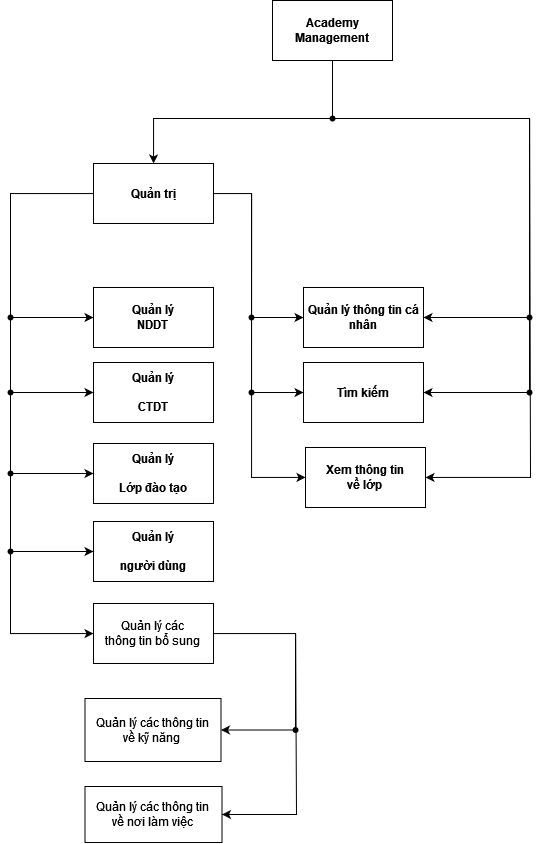
\includegraphics[height=300px]{../meta/dfd.png}
\caption{Mô hình phân rã chức năng}
\par
}
\end{figure}
\FloatBarrier

\section{Kiến trúc hệ thống}

Kiến trúc hệ thống của ứng dụng được xây dựng theo mô hình `microservice` kết hợp với mô hình client-server,
tận dụng các ưu điểm của Spring Boot để đảm bảo tính linh hoạt, khả năng mở rộng và bảo trì.

\begin{figure}[!htb]
{\centering
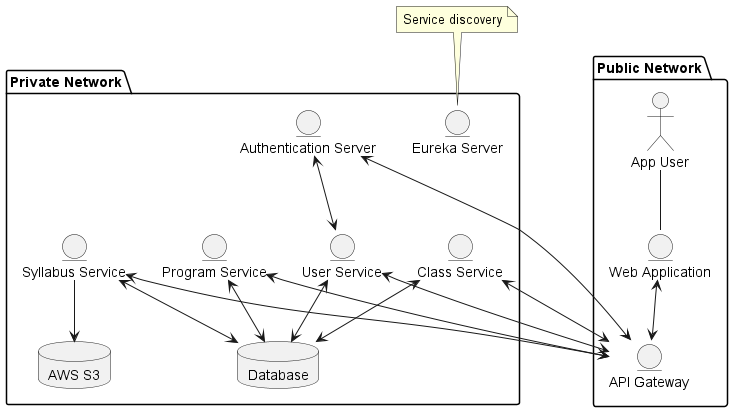
\includegraphics[width=380px]{../uml/system.arch.png}
\caption{Mô hình hệ thống}
\par
}
\end{figure}
\FloatBarrier

\subsection{Công nghệ thiết kế Backend}

\begin{itemize}[noitemsep]
  \item Spring Boot: framework Java phổ biến và dễ sử dụng để phát triển ứng dụng Java, đặc biệt là với các API và ứng dụng web.
  \item Spring Data JPA hỗ trợ các thao tác truy vấn dữ liệu với các CSDL quan hệ PostgreSQL, giúp đơn giản hóa việc truy cập và quản lý dữ liệu.
  \item Spring Security để bảo mật ứng dụng và các service, cung cấp các chức năng bảo mật như authentication và authorization (xác thực và ủy quyền).
  \item CSDL PostgreSQL
  \item Docker: sử dụng công nghệ container để đơn giản hóa việc triển khai và quản lý các service.
\end{itemize}

\begin{itemize}[noitemsep]
  \item Zipkin: Theo dõi phân tán (Distributed Tracing) giám sát và ghi lại đường đi của các request qua các service trong hệ thống phân tán, giúp người dùng có thể theo dõi và phân tích thông tin về thời gian trễ và hiệu suất của các thành phần trong hệ thống.
  \item Prometheus: giám sát thu thập số liệu của các service trong hệ thống phân tán (metrics collection)
  \item Grafana: trực quan hóa dữ liệu được thu thập bằng các biểu đồ
\end{itemize}

\textbf{Các service}:
\begin{itemize}[noitemsep]
\item Eureka: service discovery giúp các service tìm và liên lạc với nhau mà không cần hard-code host và port.
\item API Gateway: định tuyến tất cả request tới service cần thiết, ủy quyền xác thực.
\item Authentication: service xác thực thông tin người dùng, tạo, xác minh token bằng JWT (JSON Web Token).
\item User service: các API liên quan đến hoạt động quản lý user.
\item Syllabus service: các API liên quan đến hoạt động quản lý giáo trình.
\item Program service: các API liên quan đến hoạt động quản lý chương trình học.
\item Class service: các API liên quan đến hoạt động quản lý lớp học.
\item Web app: service kiến trúc client-server truyền thống để giao tiếp với user.
\end{itemize}

\subsection{Công nghệ thiết kế Frontend}

\textbf{Spring Thymeleaf} là một Java template engine được thiết kế để cho phép các lập trình viên tạo ra các giao diện người dùng bằng cách sử dụng HTML mẫu với các biểu thức động.
và được hỗ trợ bởi:

\begin{itemize}[noitemsep]
\item HTML5 và CSS: xây dựng cấu trúc và kiểu dáng cho trang web.
\item Bootstrap: framework CSS giúp cho việc thiết kế UI hiện đại, responsive và thân thiện với người dùng dễ dàng và hiệu quả hơn.
\item JavaScript: Sử dụng để viết logic bên trong các trang HTML để tăng tính tương tác.
\item jQuery: thư viện JavaScript để đơn giản hóa việc thao tác trên cây DOM HTML, xử lý event, CSS.
\item Ajax: Thư viện HTTP sử dụng trong việc tạo request đến server giúp việc lấy dữ liệu hiệu quả và dễ dàng.
\end{itemize}

\section{Mô hình Use case hệ thống}

\subsection{Use case đăng nhập}

\begin{figure}[!ht]
\caption{Mô hình use case đăng nhập}
\begin{plantuml}

@startuml

scale 401*801

left to right direction
actor User as actor

usecase "Đăng nhập" as UC
usecase "Nhập email, password" as UC1
usecase "Xác thực email, password" as UC2

actor --> UC

UC ..> UC1 : <<include>>
UC ..> UC2 : <<include>>
@enduml
\end{plantuml}
\end{figure}
\FloatBarrier

\subsection{Use Case: Quản lý nội dung đào tạo}

\begin{figure}[!ht]
\caption{Mô hình use case quản lý nội dung đào tạo}
\begin{plantuml}

@startuml

scale 401*801

left to right direction
actor User as actor

usecase "Quản lý nội dung đào tạo" as UC
usecase "Cập nhật thông tin" as UC1
usecase "Thêm nội dung đào tạo" as UC2
usecase "Thay đổi trạng thái nội dung đào tạo" as UC3
usecase "Lọc & tìm kiếm nội dung đào tạo" as UC4
usecase "Import nội dung đào tạo từ file" as UC5

actor --> UC

UC ..> UC1 : <<include>>
UC ..> UC2 : <<include>>
UC ..> UC3 : <<include>>
UC ..> UC4 : <<include>>
UC ..> UC5 : <<include>>
@enduml
\end{plantuml}
\end{figure}
\FloatBarrier

\subsection{Use case: Quản lý chương trình đào tạo}

\begin{figure}[!ht]
\caption{Mô hình use case quản lý chương trình đào tạo}
\begin{plantuml}

@startuml

scale 401*501

left to right direction
actor User as actor

usecase "Quản lý chương trình đào tạo" as UC
usecase "Cập nhật thông tin" as UC1
usecase "Thêm chương trình đào tạo" as UC2
usecase "Thay đổi trạng thái chương trình đào tạo" as UC3
usecase "Lọc & tìm kiếm chương trình đào tạo" as UC4
usecase "Import chương trình đào tạo từ file" as UC5

actor --> UC

UC ..> UC1 : <<include>>
UC ..> UC2 : <<include>>
UC ..> UC3 : <<include>>
UC ..> UC4 : <<include>>
UC ..> UC5 : <<include>>
@enduml
\end{plantuml}
\end{figure}
\FloatBarrier

\subsection{Use case: Quản lý tài liệu đào tạo}

\begin{figure}[!ht]
\caption{Mô hình use case Quản lý tài liệu đào tạo}
\begin{plantuml}

@startuml

scale 401*801

left to right direction
actor User as actor

usecase "Quản lý tài liệu đào tạo" as UC
usecase "Cập nhật thông tin" as UC1
usecase "Thêm tài liệu đào tạo" as UC2
usecase "Xóa tài liệu đào tạo" as UC3
usecase "Tải về tài liệu" as UC4

actor --> UC

UC ..> UC1 : <<include>>
UC ..> UC2 : <<include>>
UC ..> UC3 : <<include>>
UC ..> UC4 : <<include>>
@enduml
\end{plantuml}
\end{figure}
\FloatBarrier

\subsection{Use Case: Quản lý lớp đào tạo}

\begin{figure}[!ht]
\caption{Mô hình use case Quản lý lớp đào tạo}
\begin{plantuml}

@startuml

scale 401*801

left to right direction
actor User as actor

usecase "Quản lý lớp đào tạo" as UC
usecase "Cập nhật thông tin" as UC1
usecase "Thêm lớp đào tạo" as UC2
usecase "Thay đổi trạng thái lớp đào tạo" as UC3
usecase "Lọc & tìm kiếm lớp đào tạo" as UC4

actor --> UC

UC ..> UC1 : <<include>>
UC ..> UC2 : <<include>>
UC ..> UC3 : <<include>>
UC ..> UC4 : <<include>>

@enduml
\end{plantuml}
\end{figure}
\FloatBarrier

\subsection{Use case: Quản lý người dùng}

\begin{figure}[!ht]
\caption{Mô hình use case quản lý user}
\begin{plantuml}

@startuml

scale 401*801

left to right direction
actor User as actor

usecase "Quản lý thông tin tài khoản" as UC
usecase "Cập nhật thông tin" as UC1
usecase "Thêm người dùng" as UC2
usecase "Thay đổi trạng thái người dùng" as UC3
usecase "Lọc & tìm kiếm người dùng" as UC4
usecase "Import từ file" as UC5

actor --> UC

UC ..> UC1 : <<include>>
UC ..> UC2 : <<include>>
UC ..> UC3 : <<include>>
UC ..> UC4 : <<include>>
UC ..> UC5 : <<include>>
@enduml
\end{plantuml}
\end{figure}
\FloatBarrier

\subsection{Use case: Chỉnh sửa thông tin tài khoản}

\begin{figure}[!ht]
\caption{Mô hình use case chỉnh sửa thông tin tài khoản}
\begin{plantuml}

@startuml

scale 401*801

left to right direction
actor User as actor

usecase "Quản lý thông tin tài khoản" as UC
usecase "Cập nhật thông tin" as UC1
usecase "Đổi ảnh đại diện" as UC2

actor --> UC

UC ..> UC1 : <<include>>
UC ..> UC2 : <<include>>
@enduml
\end{plantuml}
\end{figure}
\FloatBarrier


\subsection{Use case: Quản lý các thông tin hỗ trợ}

\begin{figure}[!htb]
\caption{Mô hình use case quản lý phương thức đào tạo}
\begin{plantuml}

@startuml

scale 401*801

left to right direction
actor User as actor

usecase "Quản lý phương thức đào tạo" as UC
usecase "Cập nhật thông tin" as UC1
usecase "Thêm phương thức đào tạo" as UC2
usecase "Xóa phương thức đào tạo" as UC3
usecase "Tìm kiếm" as UC4

actor --> UC

UC ..> UC1 : <<include>>
UC ..> UC2 : <<include>>
UC ..> UC3 : <<include>>
UC ..> UC4 : <<include>>
@enduml
\end{plantuml}
\end{figure}
\FloatBarrier

và các mô hình usecase tương tự cho các chức năng quản lý các thông tin hỗ trợ khác như
thông tin về kỹ năng và nơi làm việc.

\section{Đặc tả use case}

\subsection{Use case đăng nhập}

% \setlength\LTleft{-2.5cm}
% \setlength\LTright{0pt plus 1fill minus 1fill}

\begin{table}[!ht]
\begin{longtable}{|p{4cm}|p{12cm}|}
\hline
\textbf{Tên usecase} & \textbf{Đăng nhập} \\
\hline
\textbf{Actor} & Người dùng quản trị \\
\hline
\textbf{Mô tả} & Người dùng đăng nhập để có thể sử dụng hệ thống \\
\hline
\textbf{Điều kiện kích hoạt} & Người dùng vào website hệ thống \\
\hline
\textbf{Tiền điều kiện} & Người dùng chưa đăng nhập vào hệ thống \\
\hline
\textbf{Hậu điều kiện} & \\
\hline
\textbf{Dòng sự kiện chính} &
\begin{itemize}[noitemsep]
  \item Hệ thống điều hướng tới trang chủ
\end{itemize}\\

\hline
\textbf{Dòng sự kiện phụ} & 
\begin{itemize}[noitemsep]
  \item Thông báo dữ liệu nhập không hợp lệ
  \item Thông báo thông tin đăng nhập không hợp lệ
\end{itemize}\\
\hline
\caption{Bảng đặc tả chức năng đăng nhập}
\end{longtable}
\end{table}
\FloatBarrier


\subsection{Use Case: Quản lý nội dung đào tạo}

\pagebreak

\begin{table}[!ht]
\begin{longtable}{|p{4cm}|p{12cm}|}
\hline
\textbf{Tên usecase} & \textbf{Quản lý nội dung đào tạo} \\
\hline
\textbf{Actor} & Nhân viên\\
\hline
\textbf{Mô tả} & Cho phép quản lý xem, thêm, xóa, sửa, tìm kiếm nội dung đào tạo \\
\hline
\textbf{Điều kiện kích hoạt} & Quản lý chọn chức năng quản lý nội dung đào tạo \\
\hline
\textbf{Tiền điều kiện} & Người dùng đã đăng nhập và có quyền quản lý \\
\hline
\textbf{Hậu điều kiện} & \\
\hline
\textbf{Dòng sự kiện chính} &
\begin{itemize}[noitemsep]
  \item Hiển thị danh sách nội dung đào tạo
  \item Người dùng chọn chức năng muốn thực hiện: xem thông tin, thêm, sửa xóa, enable nội dung đào tạo
\end{itemize}\\
\hline
\caption{Bảng đặc tả chức năng quản lý nội dung đào tạo}
\end{longtable}
\end{table}

\FloatBarrier


\subsection{Use case: Quản lý chương trình đào tạo}

\begin{table}[!ht]
\begin{longtable}{|p{4cm}|p{12cm}|}
\hline
\textbf{Tên usecase} & \textbf{Quản lý chương trình đào tạo} \\
\hline
\textbf{Actor} & Nhân viên\\
\hline
\textbf{Mô tả} & Cho phép quản lý xem, thêm, xóa, sửa, import, lọc và tìm kiếm chương trình đào tạo \\
\hline
\textbf{Điều kiện kích hoạt} & Quản lý chọn chức năng quản lý chương trình đào tạo \\
\hline
\textbf{Tiền điều kiện} & Người dùng đã đăng nhập và có quyền quản lý \\
\hline
\textbf{Hậu điều kiện} & \\
\hline
\textbf{Dòng sự kiện chính} &
\begin{itemize}[noitemsep]
  \item Hiển thị danh sách chương trình đào tạo
  \item Người dùng chọn chức năng muốn thực hiện: xem thông tin, thêm, sửa xóa, enable chương trình đào tạo
\end{itemize}\\
\hline
\textbf{Dòng sự kiện phụ} & 
\begin{itemize}[noitemsep]
  \item
\end{itemize}\\
\hline
\caption{Bảng đặc tả chức năng quản lý chương trình đào tạo}
\end{longtable}
\end{table}
\FloatBarrier

\pagebreak
\subsection{Use case: Quản lý tài liệu đào tạo}

\begin{table}[!ht]
\begin{longtable}{|p{4cm}|p{12cm}|}
\hline
\textbf{Tên usecase} & \textbf{Quản lý tài liệu đào tạo} \\
\hline
\textbf{Actor} & Nhân viên\\
\hline
\textbf{Mô tả} & Cho phép quản lý xem, thêm, xóa, sửa, tài liệu đào tạo \\
\hline
\textbf{Điều kiện kích hoạt} & Chọn chức năng xem tài liệu đào tạo bên trong nội dung đào tạo \\
\hline
\textbf{Tiền điều kiện} & Người dùng đã đăng nhập, có quyền quản lý, đã có tài liệu đào tạo \\
\hline
\textbf{Hậu điều kiện} & \\
\hline
\textbf{Dòng sự kiện chính} &
\begin{itemize}[noitemsep]
  \item Hiển thị danh sách tài liệu
  \item Người dùng chọn chức năng: xem thông tin, upload, xóa, tài liệu
\end{itemize}\\
\hline
\textbf{Dòng sự kiện phụ} & 
\begin{itemize}[noitemsep]
  \item Upload file lên AWS S3
\end{itemize}\\
\hline
\caption{Bảng đặc tả chức năng quản lý tài liệu đào tạo}
\end{longtable}
\end{table}
\FloatBarrier

\subsection{Use Case: Quản lý lớp đào tạo}

\begin{table}[!ht]
\begin{longtable}{|p{4cm}|p{12cm}|}
\hline
\textbf{Tên usecase} & \textbf{Quản lý nội dung đào tạo} \\
\hline
\textbf{Actor} & Nhân viên\\
\hline
\textbf{Mô tả} & Cho phép quản lý xem, thêm, xóa, sửa, tìm kiếm nội dung đào tạo \\
\hline
\textbf{Điều kiện kích hoạt} & Quản lý chọn chức năng quản lý nội dung đào tạo \\
\hline
\textbf{Tiền điều kiện} & Người dùng đã đăng nhập và có quyền quản lý \\
\hline
\textbf{Hậu điều kiện} & \\
\hline
\textbf{Dòng sự kiện chính} &
\begin{itemize}[noitemsep]
  \item Hiển thị danh sách nội dung đào tạo
  \item Người dùng chọn chức năng muốn thực hiện: xem thông tin, thêm, sửa xóa, enable nội dung đào tạo
\end{itemize}\\
\hline
\textbf{Dòng sự kiện phụ} & 
\begin{itemize}[noitemsep]
  \item Danh sách được refresh
\end{itemize}\\
\hline
\caption{Bảng đặc tả chức năng quản lý nội dung đào tạo}
\end{longtable}
\end{table}
\FloatBarrier



\subsection{Use case: Quản lý người dùng}

\begin{table}[!ht]
\begin{longtable}{|p{4cm}|p{12cm}|}
\hline
\textbf{Tên usecase} & \textbf{Quản lý người dùng} \\
\hline
\textbf{Actor} & Nhân viên quản trị \\
\hline
\textbf{Mô tả} & Cho phép quản lý xem, thêm, xóa, sửa, import, lọc và tìm kiếm thông tin \\
\hline
\textbf{Điều kiện kích hoạt} & Quản lý chọn chức năng \\
\hline
\textbf{Tiền điều kiện} & \\
\hline
\textbf{Hậu điều kiện} & \\
\hline
\textbf{Dòng sự kiện chính} &
\begin{itemize}[noitemsep]
  \item Hiển thị danh sách người dùng
  \item Người dùng chọn chức năng muốn thực hiện: xem thông tin, thêm, sửa xóa, đổi trạng thái của người dùng
\end{itemize}\\
\hline
\textbf{Dòng sự kiện phụ} & 
\begin{itemize}[noitemsep]
  \item Trang danh sách được update
\end{itemize}\\
\hline
\caption{Bảng đặc tả chức năng quản lý người dùng}
\end{longtable}
\end{table}
\FloatBarrier

\subsection{Use case: Quản lý thông tin tài khoản}

\begin{table}[!ht]
\begin{longtable}{|p{4cm}|p{12cm}|}
\hline
\textbf{Tên usecase} & \textbf{Quản lý thông tin tài khoản} \\
\hline
\textbf{Actor} & Người dùng quản trị \\
\hline
\textbf{Mô tả} & Người dùng có thể chỉnh sửa thông tin, mật khẩu và ảnh đại diện \\
\hline
\textbf{Điều kiện kích hoạt} & Người dùng chọn chức năng chỉnh sửa thông tin cá nhân \\
\hline
\textbf{Tiền điều kiện} &  \\
\hline
\textbf{Hậu điều kiện} & Thông tin được nhập hợp lệ \\
\hline
\textbf{Dòng sự kiện chính} &
\begin{itemize}[noitemsep]
  \item Hiển thị thông tin
  \item Người dùng chọn trường thông tin cần sửa
\end{itemize}\\
\hline
\textbf{Dòng sự kiện phụ} & 
\begin{itemize}[noitemsep]
  \item Ảnh được upload lên
  \item Thông báo thông tin nhập không hợp lệ khi nhập lỗi
\end{itemize}\\
\hline
\caption{Bảng đặc tả chức năng quản lý thông tin tài khoản}
\end{longtable}
\end{table}
\FloatBarrier

\subsection{Use Case: Import thông tin từ file}

\pagebreak %
\begin{table}[!ht]
\begin{longtable}{|p{4cm}|p{12cm}|}
\hline
\textbf{Tên usecase} & \textbf{Import file CSV} \\
\hline
\textbf{Actor} & Người dùng quản trị \\
\hline
\textbf{Mô tả} & Người dùng có thể thêm thông tin lớp học, CTDT, NDDT, user bằng cách import từ file CSV \\
\hline
\textbf{Điều kiện kích hoạt} &  \\
\hline
\textbf{Tiền điều kiện} & Người dùng chọn chức năng import \\
\hline
\textbf{Hậu điều kiện} &  Thông tin được nhập hợp lệ \\
\hline
\textbf{Dòng sự kiện chính} &
\begin{itemize}[noitemsep]
  \item Người dùng chuẩn bị file CSV đã được format hoàn chỉnh
  \item Người dùng chọn các tùy chỉnh xử lý khi thông tin được import bị trùng
\end{itemize}\\
\hline
\textbf{Dòng sự kiện phụ} & 
\begin{itemize}[noitemsep]
  \item Thông báo import lỗi hoặc import thành công
\end{itemize}\\
\hline
\caption{Bảng đặc tả chức năng import thông tin từ file CSV}
\end{longtable}
\end{table}
\FloatBarrier


\subsection{Use case: Quản lý các thông tin hỗ trợ}

\begin{table}[!ht]
\begin{longtable}{|p{4cm}|p{12cm}|}
\hline
\textbf{Tên usecase} & \textbf{Quản lý phương thức đào tạo} \\
\hline
\textbf{Actor} & Nhân viên\\
\hline
\textbf{Mô tả} & Cho phép quản lý xem, thêm, xóa, sửa, tìm kiếm PTDT \\
\hline
\textbf{Điều kiện kích hoạt} & Quản lý chọn chức năng quản lý PTDT \\
\hline
\textbf{Tiền điều kiện} & Người dùng đã đăng nhập và có quyền quản lý \\
\hline
\textbf{Hậu điều kiện} & \\
\hline
\textbf{Dòng sự kiện chính} &
\begin{itemize}[noitemsep]
  \item Hiển thị danh sách PTDT
  \item Người dùng chọn chức năng muốn thực hiện: xem thông tin, thêm, sửa xóa PTDT đào tạo
\end{itemize}\\
\hline
\textbf{Dòng sự kiện phụ} & 
\begin{itemize}[noitemsep]
  \item Danh sách PTDT được update
\end{itemize}\\
\hline
\caption{Bảng đặc tả chức năng quản lý PTDT}
\end{longtable}
\end{table}
\FloatBarrier

Tương tự cho các chức năng quản lý các thông tin hỗ trợ khác như
các thông tin về kỹ năng và nơi làm việc.

\section{Biểu đồ tuần tự}

\subsection{Use Case: Đăng nhập}

% \pagebreak
\begin{figure}[!ht]
\caption{Biểu đồ tuần tự quá trình đăng nhập}
\begin{plantuml}

@startuml

scale 401*801

actor User
participant "Web App" as w
participant "Authentication Service" as as
participant "User Service" as us
database "Database" as db

User -> w : Chọn chức năng đăng nhập
User -> w : Nhập account credentials
w -> w : Kiểm tra đầu vào
w -> as : Forward Request
as -> us : Authenticate Request
us -> db : Fetch User by email và password
db -> us : Trả về User
us -> as : Trả về Authenticated User
as -> w : Forward Response
w -> User : Login thành Công
alt đăng nhập thất bại
  db --> us : Không tìm thấy User email và password
  us --> as : forward lỗi
  as --> w : forward lỗi
  w --> w : Hiển thị lỗi sai thông tin đăng nhập
end
@enduml
\end{plantuml}
\end{figure}
\FloatBarrier

\subsection{Use Case: Quản lý nội dung đào tạo}

\begin{figure}[!ht]
\caption{Biểu đồ tuần tự quá trình quản lý nội dung đào tạo}
\begin{plantuml}

@startuml

scale 401*801

actor "User" as u
participant "Web App" as w
participant "Syllabus Service" as ss
database "Database" as db
database "AWS S3" as fs

u -> w : chọn chức năng quản lý NDĐT
w -> ss : Lấy thông tin NDĐT
ss -> db: Lấy thông tin NDĐT

db -> ss: trả về NDĐT
ss -> w: trả về NDĐT
w -> u: Hiển thị danh sách TLDT

u -> w : chức năng thêm NDĐT
w -> w : Kiểm tra Input
w -> ss : request tạo mới NDĐT
ss -> ss: Kiểm tra thông tin NDĐT
ss -> fs: Lưu tài liệu
ss -> db: Lưu vào DB
db -> ss: Lưu thành công
ss -> w: Trả về NDĐT được thêm
w -> u: Hiển thị thông báo thành công

u -> w : Chọn chức năng xóa NDĐT
w -> ss : request xóa NDĐT
ss -> ss: Kiểm tra thông tin NDĐT
ss -> fs: Xóa khỏi bucket
ss -> db: Xóa khỏi DB
db -> ss: Thành công
ss -> w: Trả về tin nhắn
w -> u: Hiển thị thông báo thành công
alt
  ss --> w: Trả về lỗi
  w --> u: Hiện thị thông báo lỗi
end

@enduml
\end{plantuml}
\end{figure}
\FloatBarrier

\subsection{Use case: Quản lý chương trình đào tạo}

\begin{figure}[!ht]
\caption{Biểu đồ tuần tự quá trình quản lý chương trình đào tạo}
\begin{plantuml}

@startuml

scale 401*801

actor "User" as u
participant "Web App" as w
participant "Program Service" as ss
database "Database" as db
database "AWS S3" as fs

u -> w : chọn chức năng quản lý CTĐT
w -> ss : Lấy thông tin CTĐT
ss -> db: Lấy thông tin CTĐT

db -> ss: trả về CTĐT
ss -> w: trả về CTĐT
w -> u: Hiển thị danh sách TLDT

u -> w : chức năng thêm CTĐT
w -> w : Kiểm tra Input
w -> ss : request tạo mới CTĐT
ss -> ss: Kiểm tra thông tin CTĐT
ss -> fs: Lưu tài liệu
ss -> db: Lưu vào DB
db -> ss: Lưu thành công
ss -> w: Trả về CTĐT được thêm
w -> u: Hiển thị thông báo thành công

u -> w : Chọn chức năng xóa CTĐT
w -> ss : request xóa CTĐT
ss -> ss: Kiểm tra thông tin CTĐT
ss -> fs: Xóa khỏi bucket
ss -> db: Xóa khỏi DB
db -> ss: Thành công
ss -> w: Trả về tin nhắn
w -> u: Hiển thị thông báo thành công
alt
  ss --> w: Trả về lỗi
  w --> u: Hiện thị thông báo lỗi
end

@enduml
\end{plantuml}
\end{figure}
\FloatBarrier

\subsection{Use case: Quản lý tài liệu đào tạo}

\begin{figure}[!ht]
\caption{Biểu đồ tuần tự quá trình quản lý tài liệu đào tạo}
\begin{plantuml}

@startuml

scale 401*600

actor "User" as u
participant "Web App" as w
participant "Syllabus Service" as ss
database "Database" as db
database "AWS S3" as fs

u -> w : chọn chức năng quản lý TLĐT
w -> ss : Lấy thông tin TLĐT
ss -> db: Lấy thông tin TLĐT

db -> ss: trả về TLĐT
ss -> w: trả về TLĐT
w -> u: Hiển thị danh sách TLDT

u -> w : chức năng thêm TLĐT
w -> w : Kiểm tra Input
w -> ss : request tạo mới TLĐT
ss -> ss: Kiểm tra thông tin TLĐT
ss -> fs: Lưu tài liệu
ss -> db: Lưu vào DB
db -> ss: Lưu thành công
ss -> w: Trả về TLĐT được thêm
w -> u: Hiển thị thông báo thành công

u -> w : Chọn chức năng xóa TLĐT
w -> ss : request xóa TLĐT
ss -> ss: Kiểm tra thông tin TLĐT
ss -> fs: Xóa khỏi bucket
ss -> db: Xóa khỏi DB
db -> ss: Thành công
ss -> w: Trả về tin nhắn
w -> u: Hiển thị thông báo thành công
alt
  ss --> w: Trả về lỗi
  w --> u: Hiện thị thông báo lỗi
end

@enduml
\end{plantuml}
\end{figure}
\FloatBarrier

\subsection{Use Case: Quản lý lớp đào tạo}

\begin{figure}[!ht]
\caption{Biểu đồ tuần tự quá trình quản lý lớp đào tạo}
\begin{plantuml}

@startuml

scale 401*801

actor "User" as u
participant "Web App" as w
participant "Class Service" as ss
database "Database" as db

u -> w : chọn chức năng quản lý lớp
w -> ss : Lấy thông tin lớp
ss -> db: Lấy thông tin lớp

db -> ss: trả về lớp
ss -> w: trả về lớp
w -> u: Hiển thị danh sách PTDT

u -> w : chức năng thêm lớp
w -> w : Kiểm tra Input
w -> ss : request tạo mới lớp
ss -> ss: Kiểm tra thông tin lớp
ss -> db: Lưu vào DB
db -> ss: Thông tin lớp được thêm
ss -> w: Trả về lớp được thêm
w -> u: Hiển thị thông báo thành công

alt
  ss --> w: Trả về lỗi
  w --> u: Hiện thị thông báo lỗi
end

@enduml
\end{plantuml}
\end{figure}
\FloatBarrier

\subsection{Use case: Quản lý người dùng}

\begin{figure}[!ht]
\caption{Biểu đồ tuần tự quá trình Lọc và tìm kiếm người dùng}
\begin{plantuml}

@startuml

scale 401*802

actor "User" as u
participant "Web App" as w
participant "User Service" as ss
database "Database" as db

u -> w : Nhập thông tin tìm kiếm
w -> ss : Gửi request
ss -> db: Tìm kiếm thông tin

db -> ss: trả về danh sách người dùng
ss -> w: forward response
w -> u: Hiển thị thông tin 

@enduml
\end{plantuml}
\end{figure}
\FloatBarrier

\subsection{Use case: Quản lý thông tin tài khoản}

\begin{figure}[!ht]
\caption{Biểu đồ tuần tự quá trình chỉnh sửa thông tin tài khoản}
\begin{plantuml}

@startuml

scale 401*802

actor "User" as u
participant "Web App" as w
participant "User Service" as ss
database "Database" as db
database "AWS S3" as s3

u -> w : Nhập thông tin tài khoản
w -> ss : request cập nhật thông tin
ss -> db: tìm thông tin
db -> ss: trả về
ss -> db: cập nhật thông tin
ss -> s3: upload ảnh đại diện
ss -> w: forward response
w -> u: Hiển thị thông tin 

@enduml
\end{plantuml}
\end{figure}
\FloatBarrier

\subsection{Use case: Quản lý các thông tin hỗ trợ}

\begin{figure}[!ht]
\caption{Biểu đồ tuần tự quá trình quản lý phương thức đào tạo}
\begin{plantuml}

@startuml

scale 401*801

actor "User" as u
participant "Web App" as w
participant "Syllabus Service" as ss
database "Database" as db

u -> w : chọn chức năng quản lý PTĐT
w -> ss : Lấy thông tin PTĐT
ss -> db: Lấy thông tin PTĐT

db -> ss: trả về PTĐT
ss -> w: trả về PTĐT
w -> u: Hiển thị danh sách PTDT

u -> w : chức năng thêm PTĐT
w -> w : Kiểm tra Input
w -> ss : request tạo mới PTĐT
ss -> ss: Kiểm tra thông tin PTĐT
ss -> db: Lưu vào DB
db -> ss: Thông tin PTĐT được thêm
ss -> w: Trả về PTĐT được thêm
w -> u: Hiển thị thông báo thành công

alt
  ss --> w: Trả về lỗi
  w --> u: Hiện thị thông báo lỗi
end

@enduml
\end{plantuml}
\end{figure}
\FloatBarrier

Tương tự cho các chức năng quản lý các thông tin hỗ trợ khác như
các thông tin về kỹ năng và nơi làm việc.

\end{document}
